\documentclass[12pt]{article}
\usepackage[utf8]{inputenc}
\usepackage{graphicx}
\usepackage{grffile}
\usepackage{color}
\usepackage[top=1in,left=1in, right = 1in, footskip=1in]{geometry}

\usepackage{tabularx}

%% \usepackage{amsmath}
\usepackage{natbib}
\usepackage{hyperref}
\bibliographystyle{plain}
\date{\today}
\thispagestyle{empty}

\usepackage{bm}

\usepackage{afterpage}
\usepackage{pdflscape}

\newcommand{\etal}{\textit{et al.}}

\newcommand{\comment}{RENEW the comment command}
\renewcommand{\comment}[3]{}
\renewcommand{\comment}[3]{\textcolor{#1}{\textbf{[#2: }\textit{#3}\textbf{]}}}

\newcommand{\jd}[1]{\comment{cyan}{JD}{#1}}
\newcommand{\swp}[1]{\comment{magenta}{SWP}{#1}}

\newcommand{\Rx}[1]{\ensuremath{{\mathcal R}_{#1}}} 
\newcommand{\Ro}{\Rx{0}}
\newcommand{\RR}{\ensuremath{{\mathcal R}}}
\newcommand{\Rhat}{\ensuremath{{\hat\RR}}}

\newcommand{\rr}{\ensuremath{{r}}}
\newcommand{\rhat}{\ensuremath{{\hat\rr}}}

\newcommand{\tsub}[2]{#1_{{\textrm{\tiny #2}}}}
\newcommand{\pEarly}{\ensuremath{\tsub{p}{early}}}

\newcommand{\figref}[1]{Fig.~\ref{fig:#1}}
\newcommand{\figlab}[1]{\label{fig:#1}}
\newcommand{\eqref}[1]{(\ref{eq:#1})}
\newcommand{\eqlab}[1]{\label{eq:#1}}
\begin{document}

\begin{flushleft}
	{\Large \textbf\newline{
		Strength and speed of an epidemic intervention
	}}
	\newline{Supplementary figure}
	\newline
	Jonathan Dushoff,
	Sang Woo Park
\end{flushleft}

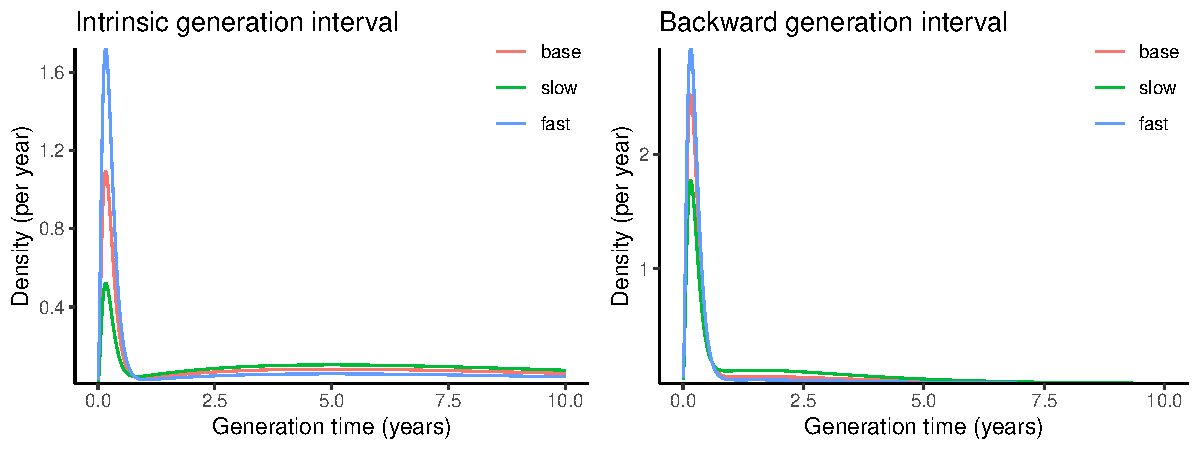
\includegraphics[width=\textwidth]{code/hivGens.Rout.pdf}

The effects of assuming slower ($\pEarly=0.1$) or faster ($\pEarly=0.4$) transmission on the intrinsic generation interval $g(\tau)$ and the initial backward generation interval $b_0(\tau)$ in our HIV scenario. Parameters as in Figure 2 from the main text.

\end{document}
